%%%%%%%%%%%%%%%%%%%%%%%%%%%%%%%%%%%%%%%%%
% Journal Article
% LaTeX Template
% Version 1.4 (15/5/16)
%
% This template has been downloaded from:
% http://www.LaTeXTemplates.com
%
% Original author:
% Frits Wenneker (http://www.howtotex.com) with extensive modifications by
% Vel (vel@LaTeXTemplates.com)
%
% License:
% CC BY-NC-SA 3.0 (http://creativecommons.org/licenses/by-nc-sa/3.0/)
%
%%%%%%%%%%%%%%%%%%%%%%%%%%%%%%%%%%%%%%%%%

%----------------------------------------------------------------------------------------
%	PACKAGES AND OTHER DOCUMENT CONFIGURATIONS
%----------------------------------------------------------------------------------------

%\documentclass[10pt]{article} % Single column

\documentclass[colorinlistoftodos,twoside,twocolumn]{article} % Two column

\usepackage{blindtext} % Package to generate dummy text throughout this template 

\usepackage[sc]{mathpazo} % Use the Palatino font
\usepackage[T1]{fontenc} % Use 8-bit encoding that has 256 glyphs
\linespread{1.05} % Line spacing - Palatino needs more space between lines
\usepackage{microtype} % Slightly tweak font spacing for aesthetics

\usepackage[spanish]{babel} % Language hyphenation and typographical rules

\usepackage[hmarginratio=1:1,top=32mm,columnsep=20pt]{geometry} % Document margins
\usepackage[hang, small,labelfont=bf,up,textfont=it,up]{caption} % Custom captions under/above floats in tables or figures
\usepackage{booktabs} % Horizontal rules in tables

\usepackage{lettrine} % The lettrine is the first enlarged letter at the beginning of the text

\usepackage{enumitem} % Customized lists
\setlist[itemize]{noitemsep} % Make itemize lists more compact

\usepackage{abstract} % Allows abstract customization
\renewcommand{\abstractnamefont}{\normalfont\bfseries} % Set the "Abstract" text to bold
\renewcommand{\abstracttextfont}{\normalfont\small\itshape} % Set the abstract itself to small italic text

\usepackage{titlesec} % Allows customization of titles
\renewcommand\thesection{\Roman{section}} % Roman numerals for the sections
\renewcommand\thesubsection{\roman{subsection}} % roman numerals for subsections
\titleformat{\section}[block]{\large\scshape\centering}{\thesection.}{1em}{} % Change the look of the section titles
\titleformat{\subsection}[block]{\large}{\thesubsection.}{1em}{} % Change the look of the section titles

\usepackage{fancyhdr} % Headers and footers
\pagestyle{fancy} % All pages have headers and footers
\fancyhead{} % Blank out the default header
\fancyfoot{} % Blank out the default footer
\fancyhead[C]{Traffic Lights Optimization} % Custom header text
\fancyfoot[RO,LE]{\thepage} % Custom footer text

\usepackage{titling} % Customizing the title section

\usepackage[colorlinks]{hyperref} % For hyperlinks in the PDF

\usepackage{graphicx} % For images

\usepackage{pifont} % bullets

\usepackage{amsmath}


% Keywords command
\providecommand{\keywords}[1]
{
	\small	
	\vspace{0.5em}
	\noindent \textbf{\textit{Palabras clave --- }} #1
}

%----------------------------------------------------------------------------------------
%	TITLE SECTION
%----------------------------------------------------------------------------------------

\setlength{\droptitle}{-4\baselineskip} % Move the title up

\pretitle{\begin{center}\Huge\bfseries} % Article title formatting
	\posttitle{\end{center}} % Article title closing formatting
\title{\normalsize{Proyecto Final Inteligencia Artificial - Simulaci\'on}\\
	\Huge\bfseries Traffic Lights Optimization\\
} % Article title
\author{% 
	\normalsize\textsc{Integrantes:}\\
	\normalsize\textsc{Leandro Rodr\'iquez Llosa}\\
	\normalsize\textsc{Laura V. Riera P\'erez}\\ 
	\normalsize\textsc{Marcos M. Tirador del Riego} \\[2ex]
	\normalsize\textsc{Grupo: C-311} \\[2ex]
	\small Tercer a\~no. Ciencias de la Computaci\'on. \\ % institution
	\small Facultad de Matem\'atica y Computaci\'on, Universidad de La Habana, Cuba \\ % institution
}
\date{\footnotesize Enero 2023 } % Leave empty to omit a date


% Abstract configurations
\renewenvironment{abstract}
{\small
	\begin{center}
		\bfseries \abstractname\vspace{-.5em}\vspace{0pt}
	\end{center}
	\list{}{
		\setlength{\leftmargin}{1.5cm}%
		\setlength{\rightmargin}{\leftmargin}%
	}%
	\item\relax}
{\endlist}


\usepackage{todonotes} % \TODO
\usepackage{listings} % Code listings
\usepackage{xcolor}
\definecolor{backcolour}{rgb}{0.95,0.95,0.92}

\newcommand{\csl}[1]{\colorbox{backcolour}{\texttt{#1}}}

\newcommand{\imgcaption}[2]{\tiny \textbf{Figura #1.} #2.}

\newcommand{\mgc}[2][]{\colorbox{backcolour}{\texttt{\_\_#2\_\_#1}}}

\newcommand{\mgccapt}[1]{\texttt{\_\_#1\_\_}}

% Hyperlinks configurations
\hypersetup{
	colorlinks=true,
	linkcolor=black,
	filecolor=magenta,      
	urlcolor=cyan,
	pdftitle={Overleaf Example},
	pdfpagemode=FullScreen,
}

%----------------------------------------------------------------------------------------

\begin{document}
	% Print the title
	\maketitle
	
	%----------------------------------------------------------------------------------------
	%	ARTICLE CONTENTS
	%----------------------------------------------------------------------------------------
	
	
	\section{Repositorio del proyecto}
	
	\begin{center}
		\href{https://github.com/science-engineering-art/traffic-lights}{https://github.com/science-engineering-art/traffic-lights}
	\end{center}
	
	\section{Descripción}
	
	En todo el mundo, la congestión del tráfico sigue siendo un problema importante en la mayoría de las ciudades, debido al creciente número de vehículos privados,  de mercancías y de transporte público. Este fenómeno afecta, sobre todo en horas pico, a los usuarios de la red vial, los cuales pierden mucho tiempo en la carretera;  además de incidir de manera negativa en el medio ambiente pues los carros se encuentran más tiempo encendidos liberando gases a la atmósfera.
	
	\vspace{0.5em}
	Se puede pensar en varias soluciones para este problema:
	\begin{enumerate}
		\item Construcción de nuevas carreteras: Muchas veces esto no es posible debido a las condiciones geográficas, y más importante aún, es muy costoso, por lo que en general no es una solución viable.
		\item Mejora del sistema de señalización vial: Es más sensata pues se relaciona inteligentemente con la infraestructura existente. Es de especial interés la mejora de los semáforos ya que estos controlan el flujo de la red vial de la ciudad. En estos podemos tener:
		\begin{itemize}
			\item Plan de luces fijo (Estático): se fijan los tiempos de verde y rojo en cada línea de luces de una intersección así como su secuencia una sola vez teniendo en cuenta las previsiones de tráfico, y estas no cambian.
			\item Controladores de tiempo real (Dinámicos): en técnicas de tiempo real, el sistema debe ser capaz de adaptarse inmediatamente (o muy brevemente) a las condiciones del tráfico. Dicho sistema posee algoritmos que permiten controlar el tráfico, los cuales reciben información sobre el estado del tráfico, que ha sido recolectada por los sensores colocados en cada carril, y recalculan la duración y la sincronización de la luces para minimizar la congestión, es decir, para minimizar el tiempo promedio de espera en las luces, y la duración de colas.
		\end{itemize} 
	\end{enumerate}

	\subsection{Objetivo}
	
	Creación de un algoritmo de control que determine el tiempo de luz verde óptimo en los semáforos de las intersecciones, con el fin de hacer más fluido el tráfico y minimizar las colas.
	
	\section{Simulación}
	
	\subsection{Modelo mesosc\'opico}
	
	Para modelar el flujo del tráfico se utiliza un modelo mesosc\'opico, modelo híbrido que combina las características de los modelos microscópico y macroscópico.
	
	Como en el modelo microsc\'opico, se representan los vehículos de forma independiente y se intenta replicar el comportamiento de un conductor. En consecuencia, es un sistema multiagente, es decir, cada vehículo opera por sí mismo utilizando información de su entorno.
	
	En cada calle (el fragmento delimitado por dos intersecciones, llamado tambi\'en cuadra), cada vech\'iculo est\'a identificado por un número i. El i-ésimo vehículo sigue al (i-1)-ésimo vehículo. Para el i-ésimo vehículo, se denota por $ x_{i} $ su posición a lo largo del camino, $ v_{i} $ su velocidad y $ l_{i} $ su longitud. Sean, adem\'as, $ s_{i} $ la distancia de parachoque a parachoque y $ \Delta v_{i} $ la diferencia de velocidad entre el i-ésimo vehículo y el vehículo que le precede (vehículo número i-1).
	
	\begin{center}
		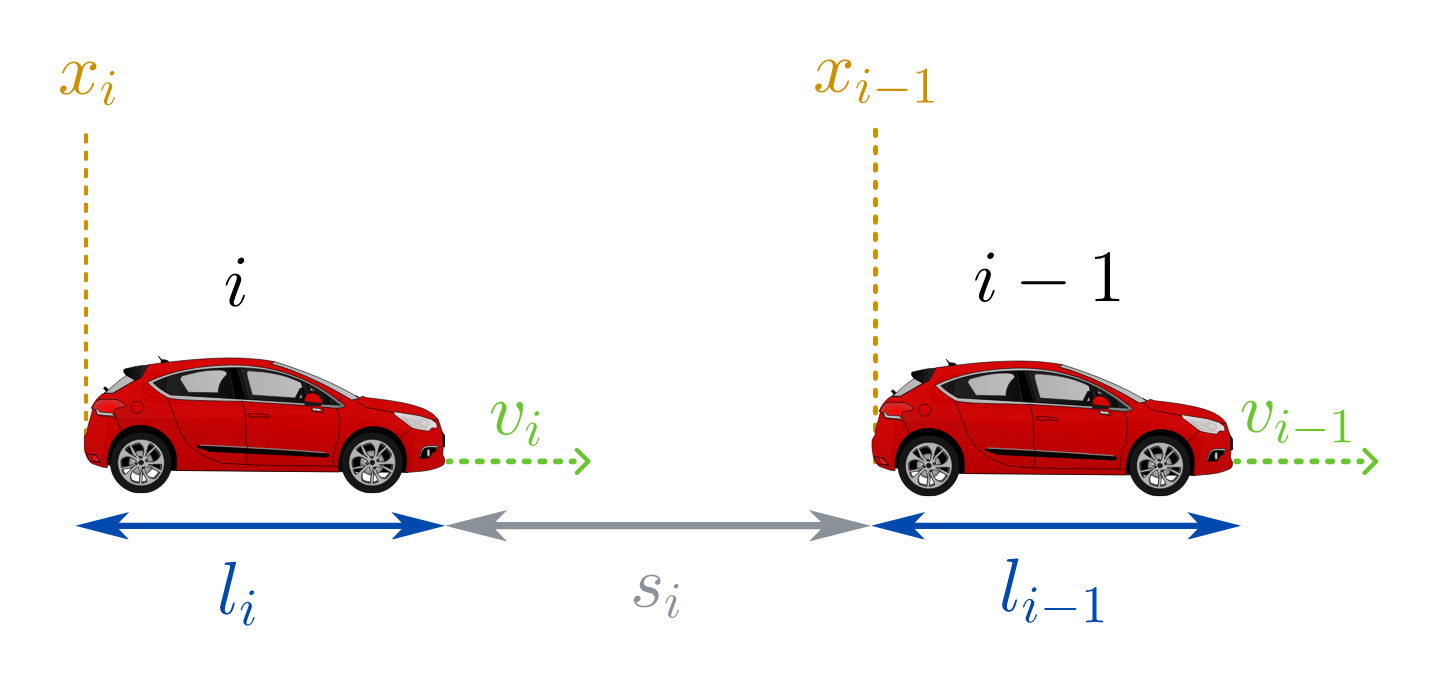
\includegraphics[width=\columnwidth]{microscopic_model.png}
	\end{center}
	
	\begin{center}
		$ s_{i} = x_{i} - x_{i-1} - l_{i} $
	
		$ \Delta v_{i} = v_{i} - v_{i-1} $
	\end{center}
	
	Por otro lado, como caracter\'istica del modelo macrosc\'opico, se tienen en cuenta factores globales que describen el movimiento de vehículos como un todo, en términos de densidad de tráfico (vehículos por km) y flujo de tráfico (vehículos por minuto), que sirven para la generación de vehículos en la simulación, que más adelante se abordará en mayor profundidad.
	
	\subsection{Modelo Conductor Inteligente}
	
	El Modelo de Conductor Inteligente\footnote{Tomado de \cite{A1}} describe la aceleración del i-ésimo vehículo en función de sus variables y las del vehículo que le precede. La ecuación dinámica se define como:
	
	\begin{center}
		$  \dfrac{dv_{i}}{dt} = a_{i} \left(1 - \left(\dfrac{v_{i}}{v_{0,i}}\right)^{\delta} - \left(\dfrac{s^{*}(v_{i}, \Delta v_{i})}{s_{i}}\right)^{2}\right)$
		
		\vspace{0.5em}
		$ s^{*}(v_{i}, \Delta v_{i}) =  s_{0,i} + v_{i}T_{i} + \dfrac{(v_{i} \Delta v_{i})}{\sqrt{(2a_{i} b_{i})}}$
	\end{center}
	donde:
	\begin{itemize}
		\item $ s_{0,i} $ : es la distancia mínima deseada entre el vehículo i el i-1.
		\item $ v_{0,i} $ : es la velocidad máxima deseada del vehículo i.
		\item $\delta$ : es el exponente de la aceleración y controla la “suavidad” de la aceleración.
		\item $ T_{i} $  : es el tiempo de reacción del conductor del i-ésimo vehículo.
		\item $ a_{i} $ : es la aceleración máxima del vehículo i.
		\item $ b_{i} $ : es la desaceleración cómoda para el vehículo i.
		\item $ s^{*} $ : es la distancia real deseada entre el vehículo i e i-1.
	\end{itemize}
	
	Interpretando los t\'erminos en $ s^{*} $:
	\begin{itemize}
		\item $ v_{i}T_{i}  $ : es la distancia de seguridad del tiempo de reacción. Es la distancia que recorre el vehículo antes de que el conductor reaccione (frene).
		Dado que la velocidad es la distancia entre el tiempo, la distancia es la velocidad por el tiempo.
		\item $ (v_{i} \Delta v_{i})/\sqrt{(2a_{i} b_{i})} $: es una distancia de seguridad basada en la diferencia de velocidad. Representa la distancia que tardará el vehículo en reducir la velocidad (sin chocar con el vehículo de enfrente), sin frenar demasiado (la deceleración debe ser inferior a $ b_{i} $).
	\end{itemize}
	
	\subsection{Modelo de red vial de tráfico}
	
	Para modelar la red vial se utiliza un grafo dirigido, donde las aristas representan las calles y los vértices las intersecciones. Cada vehículo tiene un camino que consta de múltiples calles. Se aplica el Modelo Conductor Inteligente para vehículos en la misma calle. Cuando un vehículo llega al final de la calle, se retira de la misma y es añadido a la siguiente.
	
	\subsection{Generación de vehículos}
	
	Los veh\'iculos se generan en los extremos del mapa. Cada calle tiene un $\lambda$ asignado que representa la cantidad de carros por segundo que pasan por ella, el cual corresponde a un valor entre 70 y 150 carros por hora. A las calles que se determinan como principales corresponden mayores valores de $\lambda$.
	
	Se usa $\lambda$ para saber el tiempo que se debe esperar para que pase otro carro por esta calle. Para ello se genera una variable aleatoria que cumple con la distribuci\'on  exponencial de par\'ametro lambda ($X \sim Exp(\lambda)$), cuya funci\'on de densidad es
	\begin{center}
		$f_X(x) = \lambda e^{-\lambda x}.$
	\end{center}

	Cuando haya pasado el tiempo determinado por la variable, se genera un nuevo carro en esta calle y se vuelve a generar la variable aleatoria.
	
	Al generar un carro se establece su destino y su ruta. El destino se selecciona aleatoriamente de acuerdo a una probabilidad que tiene cada calle de que un carro vaya hacia ella, asign\'andole mayor peso a las calles m\'as transitadas. Cuando se ejecuta por primera vez una simulaci\'on en un mapa, se utiliza Floyd-Warshall para hallar los caminos de menor distancia entre todo par de calles, y se guardan los mismos. La ruta de cada carro ser\'a entonces el camino de menor distancia de su calle de salida a su calle de destino, el cual est\'a precalculado.
	
	%Para la generación de vehículos se utiliza la distribución de Poisson. Esta es una distribución de probabilidad discreta, describe situaciones en las cuales los clientes llegan de manera independiente durante un cierto intervalo de tiempo y el número de llegadas depende de la magnitud del intervalo.
	
% 	\begin{center}
%		$ p(x) = f(x, \lambda) = \dfrac{\lambda^{x} \cdot e^{-\lambda}}{k!} $		
% 	\end{center}
 
	\subsection{Semáforos}
	
	\subsubsection{Turnos}
	
	Un turno es un conjunto de sem\'aforos que se encuentran en verde en un mismo per\'iodo de tiempo. Cada sem\'aforo de la intersecci\'on puede existir en m\'as de un turno, siendo posible as\'i establecer distintas combinaciones para las direcciones factibles (seguir recto, doblar a la derecha o doblar a la izquierda) tal que no haya choques y haya la menor cantidad de turnos posibles. 
	
	\subsubsection{Zonas}
	
	Los sem\'aforos tienen dos zonas en los que los veh\'iculos se comportan de forma diferente:
	\begin{itemize}
		\item Zona de ralentización: Zona en la que los vehículos reducen su velocidad máxima utilizando un factor de ralentización.
		\begin{center}
			$ v_{0,i} := \alpha v_{0,i} \hspace{0.5em} \text{donde} \hspace{0.5em} \alpha < 1$
		\end{center}
		\item Zona de parada: Zona en la que se detienen los vehículos. Esto se logra utilizando una fuerza de amortiguamiento a través de la siguiente ecuación dinámica:
		\begin{center}
			$ \dfrac{dv_{i}}{dt} = -b_{i} \dfrac{v_{i}}{v_{0,i}} $
		\end{center}
	\end{itemize}
	
	\subsection{Curvas de Bézier}
	
	Una curva de Bézier es una curva polinomial que aproxima a una serie de puntos llamados puntos de control. Est\'a definida por un conjunto de puntos de control $ P_{0} $ a $ P_{n} $ donde $ n $ es su grado. Se dice que una curva de grado n aproxima a $ n + 1 $ puntos de control. El primer y el último punto de control son siempre los puntos extremos de la curva; sin embargo, los puntos de control intermedios (si los hay) por lo general no se encuentran en la misma. 
	
	\begin{center}
		$ P(u) = \sum_{i=0}^{n} P_{i}B_{i}^{n}(u) $
	\end{center}
	\begin{center}
		$ B_{i}^{n}(u) = \binom{n}{i} (1 - u)^{n-i}u^{i} $
	\end{center}
	donde $ P_{i} $ es el conjunto de puntos, $ B_{i}^{n}(u) $ representa los polinomios de Bernstein y $ u $ toma valor entre $ 0 $ y $ 1 $.
	
	\begin{center}
		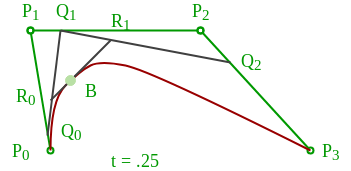
\includegraphics[width=\columnwidth]{Cubic-Bezier-Curve-Diagram}
	\end{center}
	
	Para producir una curva en nuestro mapa se crean las calles (rectas) y se utilizan las curvas de B\'ezier como un spline de suavizado. Este mismo enfoque se utiliza para crear visualmente las intersecciones, de modo que se pueda observar el giro que hace el veh\'iculo al doblar. Sin embargo si no se quiere visualizar, el veh\'iculo simplemente saldr\'a de una calle y entrar\'a en la otra, optimizando as\'i la complejidad algor\'itmica de la simulaci\'on.
	
	\section{Inteligencia Artificial}
	
	\subsection{Algoritmo genético}
	
	\subsubsection{Optimizaci\'on}
	
	Mediante el uso de un algoritmo gen\'etico se intenta minimizar la demora de los carros en las intersecciones. 
	
	\subsubsection{Proceso}
	
	El algoritmo gen\'etico consiste de varias iteraciones o generaciones. En cada iteraci\'on se tiene una poblaci\'on, o conjunto de individuos cada uno de los cuales representa una posible soluci\'on del problema. Cada poblaci\'on es el resultado de un proceso de adaptaci\'on basado en la poblaci\'on anterior. Se espera que a lo largo de las generaciones se vayan obteniendo mejores soluciones, m\'as aptas.
	
	\subsubsection{Solución}
	
	La solución (individuo) será un vector que contiene enteros correspondientes a los tiempos de luz verde de cada turno de la intersección, para todas las intersecciones del mapa. N\'otese que los tiempos de luz roja de los turnos quedar\'an determinados por la suma de los tiempos de luz verde de los restantes turnos. Se considera en este caso que la secuencia de turnos es fija y viene dada por quien provea el mapa. El vector contiene adem\'as un valor por cada intersecci\'on que corresponde a un tiempo de desplazamiento que tendr\'an los turnos de la misma. De esta forma se optimiza tambi\'en la sincronizaci\'on entre sem\'aforos. 
	
	\subsubsection{Población inicial}
	
	Para  la población inicial se genera un n\'umero fijo de individuos que componen a la misma. Cada individuo se hallará de manera aleatoria, en donde cada uno de los valores de tiempo de luz verde estará entre el tiempo promedio que le toma a un carro pasar por la intersección y el tiempo máximo que un vehículo puede estar esperando, ambos configurables. 
	
	\subsubsection{Nueva población}
	En cada iteraci\'on la nueva poblaci\'on tendr\'a la misma cantidad de individuos que la anterior. Para su creaci\'on se seleccionan algunos pares de individuos de la poblaci\'on anterior que se cruzar\'an para crear nuevas soluciones. Estas soluciones tambi\'en est\'an sujetas a mutaciones. Adem\'as, los dos individuos m\'as aptos de cada generaci\'on pasar\'an para la siguiente.   
	
	\subsubsection{Función de evaluación \textit{fitness}}
	
	Para evaluar qu\'e tan buena es una soluci\'on, se configuran los sem\'aforos de acuerdo a la misma y se ejecuta con ella un n\'umero de simulaciones (por lo general al menos 30) y se saca informaci\'on como promedio de las mismas. Luego, con los resultados arrojados por esta en un per\'iodo determinado y bajo el criterio escogido, se le da una puntuaci\'on a dicho individuo.
	
	Se consideraron tres formas de calcular el fitness:
	\begin{itemize}
		\item Seg\'un el m\'aximo, tomado sobre todas las calles, del tiempo promedio que demoran los carros transitar una una calle. 
		\item Seg\'un el tiempo total de los recorridos de todos los carros. 
		\item Seg\'un una media ponderada, tomada sobre todas las calles, del tiempo promedio que toma a los carros transitar una calle y cruzar la intersecci\'on. En este caso el peso asignado ser\'a el cuadrado de la cantidad de carros que pasan por la calle, de modo que se intenta dar mas importancia en la optimizaci\'on, a las calles m\'as transitadas. La media ponderada en cuesti\'on est\'a dada por la f\'ormula
		\[ \frac{a_1w_1^2 + a_2w_1^2 + \dots + a_nw_n^2}{w_1^2 + \dots + w_n^2},\]
	\end{itemize}
	donde $a_i$ es el tiempo que toma como promedio a los carros en la simulaci\'on cruzar la calle $i$ y $w_i$ es la cantidad de carros que la cruzan.

	N\'otese que se quieren minimizar los tiempos de los criterios anteriores, para obtener mejores soluciones. Sin embargo, dado que el algoritmo fue implementado antes buscando maximizaci\'on, se utilizan los opuestos de las m\'etricas calculadas seg\'un dichos criterios.
	
	\subsubsection{Selección de padres}
	Una de las formas de seleccionar los padres implementada fue la selecci\'on proporcional al fitness. O sea se le asigna a cada individuo una probabilidad de procrear proporcional a su fitness.
	
	Sin embargo se opt\'o mejor por la utilizaci\'on de la selección basada en el rango (\textit{rank selection}), en la cual se ordena según el valor de fitness y se da una probabilidad de selección a cada individuo. 
	
	La selección basada en el rango reduce los efectos potencialmente dominantes de individuos de alto fitness, comparativamente, en la población, estableciendo una cantidad predecible y limitada de presión de selección a favor de tales individuos. Al mismo tiempo, exagera la diferencia entre valores de fitness agrupados de forma cercana para que los mejores se puedan muestrear más.
	
	Finalmente para seleccionar los padres que van a procrear se generan aleatoriamente seg\'un la probabilidad descrita dos listas de padres, donde las parejas son los individuos en igual posici\'on de cada lista. Se tiene en cuenta que un individuo no se aparee consigo mismo. N\'otese que un individuo puede aparecer m\'ultiples veces en las listas si su probabilidad es alta, significando que deja varios descendientes. Los tama\~nos de las listas son calculados de antemano de forma que la nueva poblaci\'on sea del mismo tama\~no que la anterior.
	
	\subsubsection{Cruzamiento}
	
	La funci\'on de cruzamiento genera dos individuos para a\~nadir a la nueva poblaci\'on a partir de cada apareamiento de los padres. Se consideraron tres formas de realizar el cruzamiento:
	\begin{itemize}
		\item  \textbf{Cruzamiento por puntos m\'ultiples:} Se seleccionan p puntos random y los segmentos (resultado de picar los individuos por dichos puntos) alternos de los individuos se intercambian para obtener nuevos descendientes.
		\item \textbf{Cruzamiento geom\'etrico:} Se emparejan los genes que tienen la misma posici\'on en los padres, y en esta posici\'on del hijo se pone la media geom\'etrica entre ellos. Adem\'as de este descendiente, se devuelve uno de los padres, escogido de forma aleatoria, para que no disminuya el tama\~no de la poblaci\'on. 
		\item \textbf{Cruzamiento intermedio:} Se emparejan los genes que tienen la misma posici\'on en los padres, y en esta posici\'on del hijo se pone la media aritm\'etica entre ellos. Adem\'as de este descendiente, se devuelve uno de los padres, escogido de forma aleatoria, para que no disminuya el tama\~no de la poblaci\'on. 
	\end{itemize}
	
	\subsubsection{Mutación}
	
	La funci\'on de mutaci\'on se aplica sobre una poblaci\'on, dada una probabilidad de mutaci\'on, en este caso igual al inverso del tama\~no del vector soluci\'on. Por cada gen de cada individuo, se escoge un n\'umero $ m $ aleatorio entre $ 0 $ y $ 1 $, y dicho gen es mutado si $ m $ es menor que la probabilidad de mutaci\'on. De esta forma resulta mutado,  como promedio, un gen por cada individuo. La forma de mutar es sustituir el gen en cuesti\'on por un n\'umero aleatorio entre el tiempo promedio que le toma a un carro pasar por la intersección y el tiempo máximo que un vehículo puede estar esperando, de igual forma que para crear la poblaci\'on inicial.
	
	
	\subsection{A-star $(A^{*}) $}
	
	La b\'usqueda $ A^{*} $ es un algoritmo de búsqueda \textit{best-first} informada que utiliza la función de evaluación:
	\begin{center}
		$ f(n) = g(n) + h(n) $
	\end{center}
	donde $ g(n) $ es el costo de alcanzar el nodo $ n $, $ h(n) $ es una heur\'istica del costo estimado del camino de menor costo desde n hasta el objetivo, siendo $ f(n) $ entonces el costo estimado de la mejor soluci\'on que pasa por $ n $.
	
	Se concibieron dos algoritmos $ A^{*} $, el cl\'asico para hallar la distancia m\'inima entre dos calles, y otro para hallar el camino que menor tiempo le tomar\'a a un veh\'iculo para llegar de una calle a otra. En nuestro caso a cada nodo corresponde una esquina o intersecci\'on y a cada arista corresponde una calle que une dos intersecciones.
	
	\subsubsection{$ A^{*} $ para hallar la distancia m\'inima entre dos calles}
	
	\begin{center}
	
	\textit{$ g(n) = $ distancia recorrida hasta el momento.}
	
	\vspace{0.5em}
	\textit{$ h(n) = $ distancia en l\'inea recta desde el punto actual hasta el objetivo.}
	
	\end{center}
	
	\subsubsection{$ A^{*} $ para hallar el camino que menor tiempo le tomar\'a a un veh\'iculo para llegar de una calle a otra}
	
	\begin{center}
		\textit{$ g(n) = $ } \textit{tiempo que demor\'o el veh\'iculo en llegar desde el estado inicial hasta el \hspace{8em} estado intermedio n.}
	\end{center}	

	En este caso los valores de $g(n)$ se calculan mediante una simulaci\'on en la que el veh\'iculo va desde su posici\'on de partida hasta el punto correspondiente al nodo $n$, siguiendo el camino correspondiente al nodo $n$. Para ello se lleva una simulaci\'on del estado del tr\'ansito en la ciudad y cada vez que se quiera calcular un valor de $g(n)$, se genera un carro que hace el recorrido deseado, calculando el tiempo tomado por el mismo. Dado que el valor de $g(n) = g(m) + e$, donde $m$ es el nodo que gener\'o a $n$ y $e$ es el valor de la arista (longitud de la calle) entre ellos, este lo calculamos cuando expandimos $m$, simult\'aneamente para todos sus hijos.  

%	Para hallar $ g(n) = $ se corre una simulaci\'on con un veh\'iculo que vaya desde el estado inicial hasta el estado intermedio n, y se toma el tiempo que demor\'o en llegar a su destino. \todo{aclarar lo de que va soltando carros en cada esquina}
		
	\begin{center}
		\vspace{0.5em}
		\textit{$ h(n) = $ } \textit{aproximado del tiempo requerido para llegar del estado intermedio n \hspace{8em} hasta el estado final.}
	\end{center}

	Se precalcula antes de correr el algoritmo sobre un mapa dado, ejecutando Disjktra desde el punto de destino, de forma que se calculen para cada punto del mapa, el tiempo estimado que tomar\'a a un veh\'iculo llegar desde este hasta el destino. Para este c\'alculo se tienen en cuenta los sem\'aforos, distancia de las calles, velocidad de los carros y tr\'afico. Luego, para obtener $ h(n) $ simplemente se busca el tiempo precalculado correspondiente al punto del mapa relativo al nodo $n$.
	

	\section{Tests}
	
	Se ejecutaron 53 pruebas con los siguientes par\'ametros para la optimizaci\'on:
	\begin{itemize}
		\item \textbf{tama\~no de la poblaci\'on:} 30,
		\item \textbf{cantidad de iteraciones:} 50,
		\item \textbf{tiempo de observaci\'on de cada individuo en la simulaci\'on:} 10s,
		\item \textbf{velocidad de la simulaci\'on:} 30, que significa que por cada segundo en tiempo real, habr\'an pasado 30s en el entorno simulado,
		\item \textbf{tipo de cruzamiento:} cruzamiento por puntos m\'ultiples (2),
		\item \textbf{c\'alculo de fitness:} seg\'un la media ponderada, calculada sobre todas las calles, del tiempo promedio que toma a los carros cruzar una calle,
		\item \textbf{tiempo promedio que le toma a un carro pasar por la intersección:} 3s,
		\item \textbf{tiempo máximo que un vehículo puede estar esperando:} 90s,
	\end{itemize}
	sobre el mapa, de $ 12 \times 6 $ cuadras y $ 29 $ intersecciones semaforizadas, que se muestra a continuaci\'on:
	
	\begin{center}
		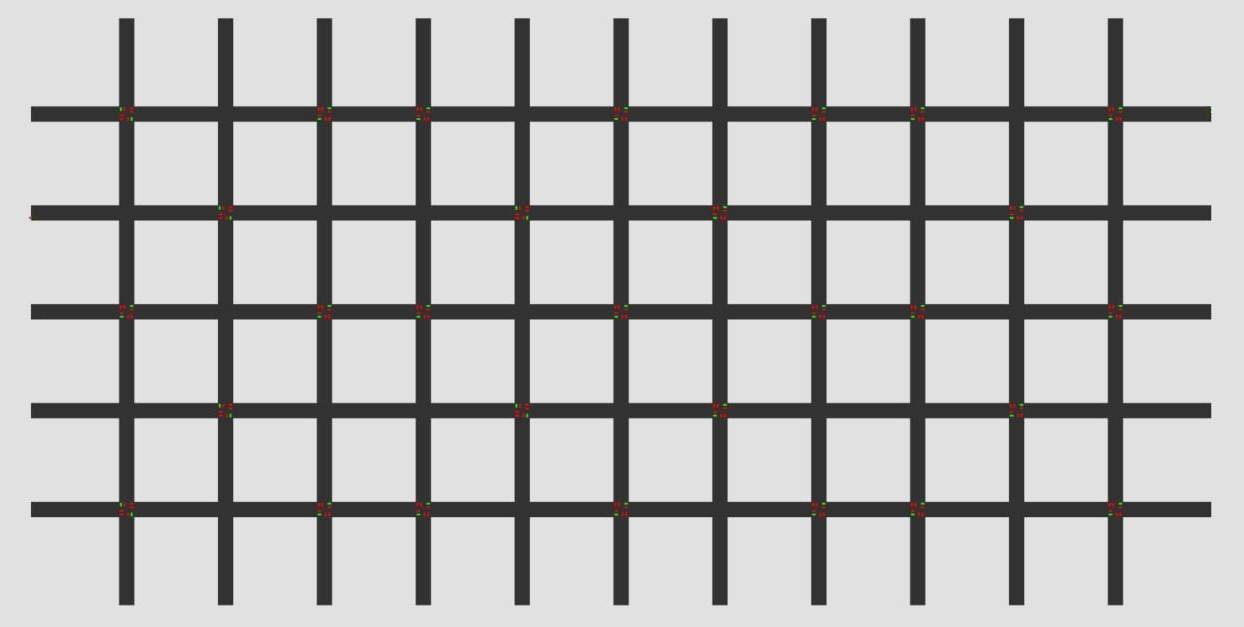
\includegraphics[width=\columnwidth]{map.jpg}
	\end{center}
	
	Dichas pruebas se pueden encontrar en la carpeta \emph{tests} del repositorio. 

	\subsection{Resultados}
	
	La siguiente gr\'afica muestra los valores de fitness de las 53 pruebas corridas del algoritmo gen\'etico. Se puede observar que el valor de fitness en la mayor\'ia de los tests, para la mejor soluci\'on obtenida, se mantiene en el rango de 23 a 26. Esto podr\'ia interpretarse como que los carros (sobre todo aquellos en las calles m\'as transitadas porque les dimos mayores pesos) se demoran como promedio $25s$ en cruzar una calle. Hay que notar que hubo algunos tests cuyas mejores soluciones dieron valores demasiado buenos para ser reales, los cuales fueron marcados en rojo y naranja en la gr\'afica. Los resultados marcados en naranja es probable que se deban a que la aleatoriedad haya como resultado simulaciones muy perfectas, por casualidad, mientras que los marcados en rojo deben haber sido errores ocurridos durante la ejecuci\'on del algoritmo.
	
	\begin{center}
		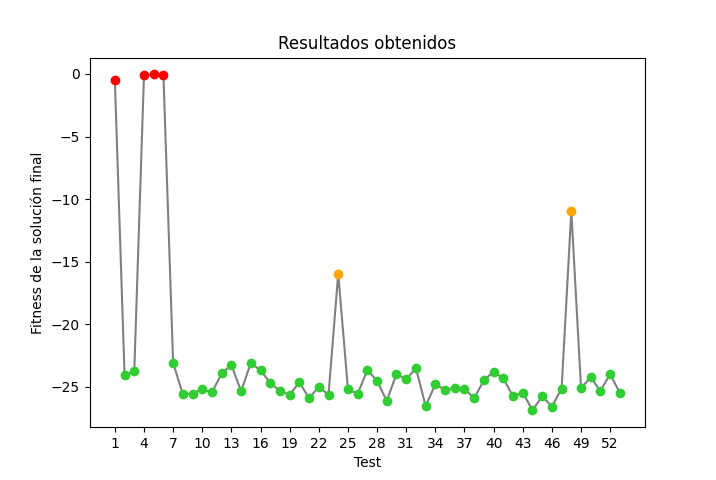
\includegraphics[width=\columnwidth]{graphic_resultados_obtenidos.png}
	\end{center}

	Observando los valores de fitness obtenidos para cada test, a lo largo de todas las generaciones, se puede notar que estos tienen siempre tendencia a mejorar. Para apreciar mejor esto, se provee junto con este trabajo un gr\'afico por cada test, donde se muestran para cada generaci\'on, la mejor y peor soluci\'on, pudiendo apreciar claramente como la curva que describen es creciente. La siguiente gr\'afica muestra una uni\'on de todas las gr\'aficas antes descritas, para todos los tests. En ella se puede ver claramente como los valores de fitness van aumentando seg\'un pasan las generaciones.

	\begin{center}
		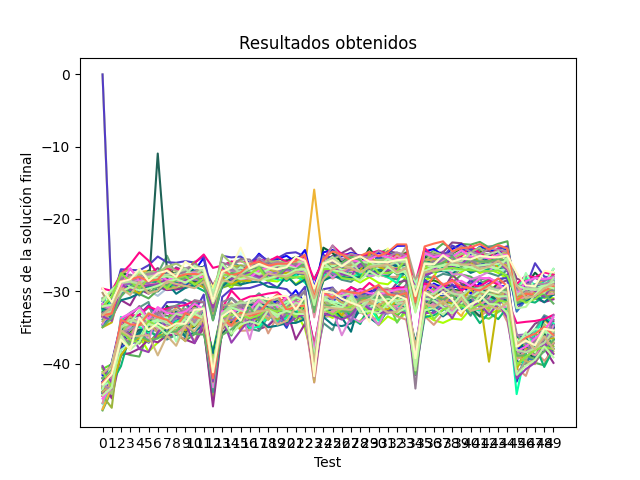
\includegraphics[width=\columnwidth]{all_graphics.png}
	\end{center}

	Finalmente, se seleccionaron por cada test las mejores soluciones y alguna soluci\'on arbitraria de la primera generaci\'on. Para estas se calcularon nuevamente, mediante algunas ejecuciones m\'as de la simulaci\'on, el tiempo total que toma a todos los veh\'iculos en completar su recorrido en el mapa. En la gr\'afica a continuaci\'on se muestran en puntos azules las mejores soluciones, y en rojo las de la primera generaci\'on. Se puede apreciar que los puntos azules se encuentra siempre por encima de los rojos, llegando a encontrarse diferencias de hasta m\'as de una hora (entre todos). Teniendo en cuenta que las simulaciones fueron realizadas durante $5$ minutos solamente, una mejor\'ia de una hora en los pocos carros que pueden haber circulado el mapa en este tiempo, nos da una medida de qu\'e tanto se podr\'ia llegar a optimizar si se ejecuta el tiempo suficiente.
	
	\begin{center}
		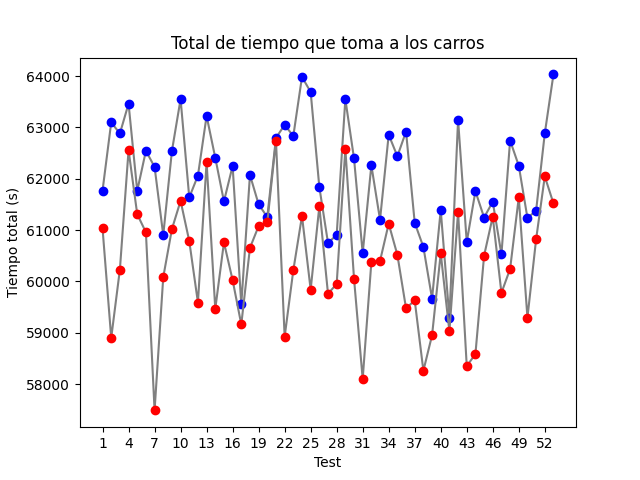
\includegraphics[width=\columnwidth]{graphic_total_time_take_cars.png}
	\end{center}

	Como conclusi\'on podemos decir que el algoritmo arroja resultados que optimizan en cierta medida el tiempo de demora de los carros en su trayecto. Hay que tener en cuenta que dada la limitada capacidad de c\'omputo con que se contaba, y el poco tiempo del que se dispuso para obtener los resultados, se tuvieron que relajar mucho los par\'ametros utilizados. Idealmente deber\'ian haberse corrido simulaciones m\'as largas y con un tama\~no de poblaci\'on m\'as acorde al n\'umero de coordenadas de los vectores soluci\'on.

	\section{Recomendaciones}
	
	Se recomienda, con m\'as tiempos y capacidad de c\'omputo, correr el algoritmo gen\'etico con par\'ametros m\'as grandes. Pudiera tambi\'en escalarse el mapa para simular una ciudad m\'as grande. Otra recomendaci\'on es probar con otras m\'etricas para optimizar necesidades m\'as espec\'ificas de un posible cliente.
	
	Como trabajo futuro ser\'ia interesante hacer que la distribuci\'on de los turnos formase parte de la soluci\'on, de forma que una distribuci\'on dada pueda contribuir a un mejor flujo del tr\'afico. Tambi\'en se pudiera optimizar la posici\'on de las intersecciones semaforizadas (a\~nadir, quitar o reacomodar intersecciones en el mapa), para contribuir a hacer el tr\'afico m\'as fluido, objetivo perseguido en este proyecto.
	
	Tambi\'en se recomienda quitar algunas de las relajaciones realizadas al problema para simular un ambiente m\'as parecido  a uno real. Por ejemplo, incluir el t\'rafico de peatones o permitir que los carros cambien de senda a antojo del conductor.
	
	La generación de mapas, se hace de una manera determista, y por cada mapa se tiene que implementar un template que lo construya. Este proceso de generación se puede automatizar utilizando una grámatica libre del contexto con algún tipo de conocimiento asociado a la modelación de un mapa. Por ejemplo se conoce que si se tiene una calle principal, la calle que le sigue forma parte de la calle principal y conserva el mismo número de carriles, y las calles que la cruzan por lo general no son avenidas principales ya que estas se encuentran dispersas. Pero como las producciones de una gramática libre del contexto son determinitas quizás puedan caer en el mismo problema que se tenía inicialmente, o sea, construir mapas de un tipo específico. Entonces se puede pensar en en a\~nadir a cada producción una probabilidad asociada que le de mayor peso a producciones correspondientes a distribuciones de calles que tiene m\'as ocurrencia en la vida real y menos a las que no. Finalmente, lo que se está proponiendo es utilizar una gramática libre del contexto probabilística para poder generar mapas arbitrarios sin tener que generar un template por cada mapa distinto que se quiera obtener.

\begin{thebibliography}{20}
	\bibitem{A1} Martin Treiber, Ansgar Hennecke, and Dirk Helbing: \emph{Congested traffic states in empirical observations and microscopic simulations}. Phys. Rev. E 62, 1805 – Published 1 August 2000.
	\bibitem{russel} Martin Treiber, Ansgar Hennecke, and Dirk Helbing: \emph{Congested traffic states in empirical observations and microscopic simulations}. Phys. Rev. E 62, 1805 – Published 1 August 2000.
\end{thebibliography}
\todo{Agregar bibliografia}
\end{document}

